\documentclass[a4paper, 12pt]{article}

\usepackage[portuges]{babel}
\usepackage[utf8]{inputenc}
\usepackage[T1]{fontenc}
\usepackage{times} % Fonte Times New Roman
\usepackage{setspace}
\usepackage{mathptmx} 
\onehalfspacing
\usepackage{amsmath}
\usepackage{indentfirst}
\usepackage{graphicx}
\usepackage{multicol,lipsum}
\usepackage{enumitem}
\usepackage{url}
\usepackage{booktabs}
\usepackage{array}
\usepackage{tocloft}
\usepackage{fancyhdr}
\usepackage[a4paper, 
            left=3cm,    
            right=2cm,   
            top=3cm,    
            bottom=2cm   
            ]{geometry}


\begin{document}
%\maketitle

\begin{titlepage}
	\begin{center}
	
	\begin{figure}[!ht]
	\centering
	
\includegraphics[width=10cm]{Logo Transparente Preto.png} \\ 
    \end{figure}

        
		\vspace{115pt}
        \textbf{\Huge{Aplicativo para engajamento comunitário}}\\
		%\title{{\large{Título}}}
        
		\vspace{115pt}
        Carlos Eduardo Nogueira Silva \\
        Felipe Gomes da Silva \\
        Felipe Matheus Possari \\
        Matheus Thomé da Silva\\ 
        Santiago Pinheiro Martins \\
	\end{center}
	
	
	\vspace{1cm}
	\begin{center}
		\vspace{\fill}
		 Abril \\
		 2025
			\end{center}
\end{titlepage}
%%%%%%%%%%%%%%%%%%%%%%%%%%%%%%%%%%%%%%%%%%%%%%%%%%%%%%%%%%%




\newpage
\thispagestyle{empty}
\tableofcontents

\newpage 
\thispagestyle{empty}
\listoffigures

\newpage
\thispagestyle{empty}
\listoftables

\newpage
\pagestyle{fancy}

\fancyhead[L]{\thepage}
\fancyhead[C]{\nouppercase{\leftmark}}
\rhead{
\includegraphics[width=2cm]{Logo Transparente Preto.png}}
\fancyfoot[R]{}
\fancyfoot[C]{© 2025 - PuSystems}
\fancyfoot[L]{}
\setlength\headheight{26pt}

% % % % % % % % % % % % % % % % % % % % % % % % % % %
\section{Introdução}
O município de São José do Rio Preto está lidando com uma das mais graves epidemias de dengue já registradas no estado, com mais de 35.000 casos confirmados da enfermidade apenas em 2025, posicionando-se como a cidade com maior probabilidade de casos em todo o Brasil. Conquanto haja esforços das autoridades públicas para conscientizar a população, essa epidemia ainda parece longe de cessar. Deste modo, uma urbanização adequada e a eliminação de focos do mosquito da dengue, com o esforço público, fazem-se necessárias.

Destaca-se a importância da população na luta contra o mosquito, sendo o único grupo capaz de identificar facilmente os focos de dengue em sua residência e arredores. Portanto, o objetivo da PuSystem é capacitar os habitantes de São José do Rio Preto para que eles mesmos possam aprimorar a condição da cidade e se empenhem para isso.

Para estimular a participação, o sistema se baseará no modelo de \textit{gamificação} Octalysis, criado pelo escritor e empresário Yu-Kai Chou.  O modelo Octalysis é empregado na criação de sistemas de \textit{gamificação} destinados a potencializar a motivação humana.  Ele alcança esse objetivo ao reconhecer oito "impulsos principais" que precisam ser estimulados:

\begin{enumerate}
    \item \textbf{Epic Meaning \& Calling} se refere à motivação em participar de algo que consideramos maior que nós mesmos, tomando partido em uma causa nobre ou propósito grandioso com impacto importante a nossa vizinhança, cidade, país ou mundo. 
    \item \textbf{Development \& Accomplishment} é o desejo de melhorar, crescer e conquistar. Refere-se à motivação que obtemos ao avançar em direção a algum objetivo e superarmos obstáculos e alcançarmos marcos, seja em habilidades, conquistas ou metas pessoais.
    \item \textbf{Empowerment of Creativity \& Feedback} é a motivação que surge da chance de criar, experimentar e observar as consequências de suas ações. As pessoas se sentem estimuladas quando possuem liberdade para explorar e fazer suas próprias escolhas. 
    \item \textbf{Ownership \& Possession} é o impulso que temos ao percebermos que possuímos responsabilidade sobre algo, seja um projeto, ideia ou objetivo. Nos sentimos mais estimulados ao investir tempo e esforço para preservar e aprimorar o que consideramos nosso
    \item \textbf{Social Influence \& Relatedness} é a motivação social e ocorre através do contato com outras pessoas. Indivíduos se sentem estimulados a aderir a grupos ou  obter o apoio de seus colegas. 
    \item \textbf{Scarcity \& Impatience} está intimamente ligado à percepção de valor que aumenta quando a disponibilidade de um item ou recurso é restrita. Além disso, a frustração causada pela espera ou pela falta de acesso a esses recursos escassos pode gerar um impulso emocional mais intenso para obtê-los.
    \item \textbf{Unpredictability \& Curiosity} explora a imprevisibilidade presente em uma experiência, como surpresas e enigmas a serem desvendados, como uma forte fonte de motivação. Quando há dúvidas sobre o futuro, as pessoas costumam se envolver mais para satisfazer sua curiosidade e prever o que está por vir.
    \item \textbf{Loss \& Avoidance} é a motivação que origina da vontade de evitar danos ou prejuízos, fazendo uso do instinto de protegermos aquilo que já possúimos, como um recurso, posição ou vantagem.
\end{enumerate}

Seguindo tais principios, o objetivo da PuSystems é desenvolver um sistema que incentive todos os elementos motivacionais na população de São José do Rio Preto, permitindo que eles se conscientizem sobre sua própria saúde, entendam o ciclo de vida do Aedes aegypti e do vírus da dengue, além de agirem eliminando focos de proliferação e acionando as autoridades em situações de emergência. Cada um dos 8 focos estará associado a requisitos funcionais citados no capitulo \ref{sec:requisitos}.

\newpage
\section{Especificação de Requisitos}\label{sec:requisitos}

A documentação clara e organizada das necessidades, funcionalidades e limitações de um sistema ou projeto é chamada de especificação de requisitos.  A meta é chegar a um consenso entre os interessados, assegurando que o produto final cumpra as expectativas e exigências técnicas.  Este passo é crucial no processo de desenvolvimento, pois estabelece a fundação para o design, a implementação e a validação.  Emprega métodos como a coleta de requisitos funcionais, não funcionais e casos de uso, garantindo exatidão e abrangência.  Uma descrição adequada minimiza ambiguidades e diminui os custos de retrabalho. Desta forma, o sistema desenvolvido deverá conter:

\subsection{Registro e Gestão de Usuários}
\begin{enumerate}
    \item Registro de um perfil personalizado, com os seguintes campos: nome social, documento oficial, foto de perfil, gênero, idade, endereço (bairro) e foco no combate à dengue.
    \item Exigência de login com senha e documento oficial e senha para acesso aos recursos do aplicativo.
    \item Possibilidade de atualização dos dados cadastrais.
\end{enumerate}

\subsection{Módulo Educacional}
\begin{enumerate}
    \item Conteúdo organizado em diferentes cursos/módulos para melhor absorção e aprendizado.
    \item \textit{Player} de vídeos para vídeo-aulas, com suporte a legendas.
    \item Transmissões ao vivo para anúncios oficiais em palestras de temas relevantes
    \item Tutoriais multimídias (textos, vídeos e \textit{quizzes}) que ensinam a identificar e eliminar focos de mosquito da dengue.
\end{enumerate}

\subsection{Sistema de \textit{Gamificação}}
\begin{enumerate}
    \item Um score pessoal para cada usuário registrado.
    \item Ranking geral e por bairro mostrando a classificação de todos os usuários, incentivando uma competição de maneira saudável.
    \item Destaque para os usuários de com maior ganho de pontuação na página principal.
    \item Conquistas pessoais associadas a realização de ações incentivadas um número específico de vezes.
    \item Histórico de conquista onde cada usuário poderá visualizar suas próprias conquistas, estatísticas e a de outros usuários.
    \item Missões individuais aleatórias como assistir um número determinado de aulas, realizar ou eliminar um número específicos de focos, etc.
    \item Missões cooperativas como reduzir o número de casos reportados ou focos denunciados, elevando o score da região.
    \item Recompensas como ganho de pontos e conquistas ao concluir missões e realizar ações incentivadas.
    \item Penalidades como perda de pontos por inatividade.
    \item Recompensas surpresa ao preencher o registro de sintomas ou consumir conteúdo educacional regularmente, como pontos extras ou conquistas especiais.
    \item Geração de missões de tempo limitado, com tarefas especiais surgindo por um período curto.
\end{enumerate}

\subsection{Sistema de Denúncias e Monitoramento de Áreas de Risco}
\begin{enumerate}
    \item Formulário de denúncia de focos de mosquito, incluindo texto, foto e localização.
    \item Envio automático de denúncias para a equipe responsável para que validem e atualizem o status do foco. 
    \item Exibição de áreas de risco no mapa, utilizando dados climáticos, registros de casos e localização de denúncias para indicar regiões com maior incidência.
    \item Envio de notificações ao usuário sobre aumento de casos em sua região ou surgimento de focos próximos ao seu endereço.
    \item Envio de notificações sobre a pontuação do bairro, informando se está melhorando ou piorando com base no engajamento comunitário.
\end{enumerate}

\subsection{Sistema de Monitoramento de Sintomas}
\begin{enumerate}
    \item Um questionário simples com perguntas sobre febre, dor de cabeça, dores musculares e outros sintomas característicos da dengue que pode ser preenchido periodicamente
    \item Alertas de suspeita, caso os sintomas sejam compatíveis com a doença, indicando a necessidade de buscar atendimento médico e informando as autoridades de saúde.
\end{enumerate}
\subsection{Gerenciamento e Suporte a Autoridades}
\begin{enumerate}
    \item Painel de estatísticas permitindo que autoridades monitorem as informações geoespaciais da cidade e bairros, as denúncias de focos e o número de casos  reportados
    \item Painel para a avaliação e atualização dos status de denúncias realizadas.
    \item Integração com sistema oficiais para que dados sobre surtos, casos e relatórios de saúde pública possam ser importados.
\end{enumerate}

\newpage
\section{Plano de Projeto}

\subsection{Introdução}
% descreve os objetivos gerais do trabalho e restrições que afetam a gerência do projeto

\subsection{Organização do Projeto}
% descreve o modo como a equipe de desenvolvimento é organizada, as pessoas envolvidas e seus papéis na equipe

\subsection{Análise de Riscos}
% descreve possíveis riscos de projeto, a probabilidade de surgir tais riscos e as estratégias propostas para a sua redução

A avaliação de riscos consiste em um procedimento sistemático para detectar, avaliar e atenuar potenciais ameaças que possam afetar metas, projetos ou operações. Inclui a identificação de cenários desfavoráveis, a probabilidade de sua ocorrência e a severidade das consequências. Este método é fundamental em campos como engenharia, administração de projetos e segurança da informação, possibilitando decisões fundamentadas em provas. A abordagem mescla métodos qualitativos e quantitativos para destacar medidas preventivas e corretivas, minimizando incertezas e vulnerabilidades.

\subsubsection{Metodologia de Análise de Riscos}

Para o desenvolvimento adequado do projeto e propor estratégias com o fim de mitigar os principais riscos que podem comprometer o sucesso do projeto, adotamos a metodologia da análise qualitativa de riscos, na qual valores são atribuídos aos riscos para identificar o impacto potencial desses itens nos resultados possíveis. Assim, a avaliação é baseada nos seguintes critérios:

\begin{itemize}
    \item \textbf{Probabilidade (P):} Baixa (1), Média (2), Alta (3)
    \item \textbf{Impacto (I):} Baixo (1), Médio (2), Alto (3)
    \item \textbf{Nível de Risco (R):} R = P × I
    \item \textbf{Classificação:}
    \begin{itemize}
        \item Baixo (1 a 2)
        \item Moderado (3 a 4)
        \item Alto (6 a 8)
        \item Crítico (9)
    \end{itemize}
\end{itemize}

\subsubsection{Riscos Identificados}
A Tabela \ref{tab:risks} apresenta os principais riscos identificados no projeto, contemplando suas causas, potenciais impactos e estratégias iniciais de mitigação. Esta análise preliminar visa antecipar desafios críticos que poderiam comprometer prazos, custos ou qualidade do produto. 

\begin{table}
\caption{Riscos Identificados}
\label{tab:risks}
\begin{tabular}{|c|p{4cm}|c|c|c|p{5.7cm}|}
\hline
\textbf{ID} & \textbf{Risco} & \textbf{P} & \textbf{I} & \textbf{R} & \textbf{Estratégia} \\
\hline
R1 & Baixa adesão da população ao aplicativo & 2 & 3 & 6 (Alto) & Campanhas de conscientização, foco em UX e gamificação. \\
\hline
R2 & Denúncias falsas & 2 & 3 & 6 (Alto) & Validação por autoridades; penalidades para abuso. \\
\hline
R3 & Perda de dados ou vazamento & 2 & 3 & 6 (Alto) & Implementar criptografia AES-256, seguindo a LGPD. \\
\hline
R4 & Resistência de autoridades à adoção do sistema & 2 & 3 & 6 (Alto) & Envolver representantes da saúde pública nas etapas iniciais. Treinamentos e demonstração de benefícios. \\
\hline
R5 & Desinteresse após uso inicial (retenção de usuários) & 3 & 3 & 9 (Crítico) & Missões dinâmicas, notificações personalizadas, recompensas variadas e surpresas. \\
\hline
R6 & Difícil obtenção de dados climáticos e epidemiológicos em tempo real & 2 & 2 & 4 (Moderado) & Utilizar, bibliotecas, APIs e fontes públicas confiáveis, com fallback offline. \\
\hline
R7 & Desistência de membros da equipe durante o projeto & 1 & 3 & 3 (Moderado) & Garantir divisão de tarefas e documentação. \\
\hline
R8 & Falha no sistema de gamificação & 2 & 3 & 6 (Alto) & Testes rigorosos e feedback contínuo dos usuários\\
\hline
R9 & Dependência excessiva de autoridades para validar denúncias & 3 & 2 & 6 (Alto) & Automatizar validações com IA (ex.: análise de fotos) e capacitar equipes locais. \\
\hline
R10 & Falha na integração com sistemas oficiais de saúde & 2 & 3 & 6 (Alto) & APIs robustas, parcerias prévias com órgãos públicos, plano de contingência manual. \\
\hline
R11 & Conteúdo educacional ineficaz ou desatualizado & 1 & 2 & 2 (Baixo) & Revisão periódica por especialistas em saúde; feedback dos usuários. \\
\hline
R12 & Sobrecarga de servidores devido ao alto tráfego & 2 & 3 & 6 (Alto) & Infraestrutura escalável (cloud computing) e monitoramento em tempo real. \\
\hline
R13 & Viés em rankings (ex.: bairros mais pobres com menos engajamento) & 2 & 3 & 6 (Alto) & Adaptar critérios de pontuação por contexto socioeconômico e missões equilibradas. \\
\hline
R14 & Falha no monitoramento de sintomas  & 2 & 3 & 6 (Alto) & Revisão por médicos e alertas sobre limitações. \\
\hline
\end{tabular}
\smallskip
Elaborado pelos autores (2025).
\end{table}

\newpage
\subsubsection{Plano de Ação para Riscos Críticos}

Para os riscos classificados como \textbf{alto impacto} (R $\geq$ 6) e \textbf{críticos} (R = 9), serão adotadas as seguintes ações prioritárias:

\begin{itemize}
    \item \textbf{R1 (Baixa adesão):} Desenvolver MVP com foco em gamificação e realizar testes de usabilidade com moradores de diferentes perfis socioeconômicos.
    \item \textbf{R2 (Denúncias falsas):} Implementar sistema de verificação em duas etapas: análise automatizada de fotos por meio de IA e validação manual amostral.
    \item \textbf{R3 (Vazamento de dados):} Adotar autenticação OAuth2, criptografia AES-256 para dados sensíveis e auditorias de segurança bimestrais.
    \item \textbf{R4 (Resistência de autoridades):} Criar comitê consultivo com representantes da vigilância sanitária municipal desde a fase de prototipagem.
    \item \textbf{R5 (Desinteresse pós-uso):} Designar um "gamification owner" na equipe para atualizar semanalmente missões e recompensas surpresa.
    \item \textbf{R8 (Falhas na gamificação):} Implementar sistema A/B testing para mecânicas de pontuação e criar ambiente sandbox para testes antes do deploy.
    \item \textbf{R9 (Dependência de autoridades):} Capacitar agentes comunitários de saúde como validadores secundários via aplicativo dedicado.
    \item \textbf{R10 (Integração com sistemas):} Estabelecer parceria formal com a Secretaria Municipal de Saúde para acesso a APIs oficiais de dados epidemiológicos.
    \item \textbf{R12 (Sobrecarga de servidores):} Configurar auto-scaling na AWS com monitoramento contínuo via CloudWatch e plano de contingência para picos.
    \item \textbf{R13 (Viés em rankings):} Desenvolver algoritmo de ponderação que considere indicadores socioeconômicos do IBGE por região.
    \item \textbf{R14 (Falsos sintomas):} Integrar sistema com protocolos clínicos oficiais do Ministério da Saúde e incluir disclaimer médico nos alertas.
\end{itemize}

\subsubsection{Monitoramento Contínuo}
    Será realizada uma revisão trimestral do risk register pelo comitê que reune a equipe técnica e os representantes da saúde pública de São José do Rio Preto com a finalidade de levantar os dados sobre os riscos e manter o aplicativo funcional e com boa performance. 
    Um relatório mensal de eficácia das ações mitigatórias também será feito, além da crição de dashboard de riscos para uma melhor compreensão do progresso da aplicação, contendo indicadores como: 
    \begin{itemize}
        \item Número de denúncias validadas/invalidadas
        \item Taxa de engajamento por bairro
        \item Tempo médio de resposta das autoridades
        \item Incidentes de segurança registrados
    \end{itemize}
    Além disso haverá atualização dos níveis de risco após cada release importante do aplicativo.



\subsection{Requisitos de Apoio de Hardware e Software}
% descreve o hw e o sw de apoio exigidos para realizar o desenvolvimento. 
% Se o hw precisar ser comprado, incluir prazos de entrega e estimativas de preço

Para obter-se o melhor resultado na produção deste software, precisa-se analisar quais são os sistemas de apoio, tanto físicos quanto lógicos necessários. No geral, o desenvolvimento, pela parte da PuSystems, não precisara de uma grande massa de recursos, estes estarão ou armazenados em outros servidores, ou na própria borda do sistema, no usuário final. 

Estes, a seguir, são comportamentos esperadas do sistema, baseados nos requisitos funcionais: 

\subsubsection{Desempenho e Qualidade}
\begin{itemize}[]
  \item Velocidade: Páginas principais devem carregar em até 200ms.
  \item Disponibilidade: Sistema online 24/7.
  \item Segurança: Criptografia avançada dos dados sensíveis.
  \item Usabilidade: Usuário deve se adaptar em até 2 horas através de uma UI simples e intuitiva.
\end{itemize}

O sucesso do projeto depende de uma infraestrutura adequada e da adoção de padrões técnicos claros. Para garantir eficiência, segurança e escalabilidade, foram definidos os seguintes requisitos:

\subsubsection{Tecnologia e Ferramentas}
\begin{itemize}[]
\item Front-end: React Native com TypeScript (para desenvolvimento multiplataforma).
\item Back-end: Node.js + Express.js, com PostgreSQL para armazenamento de dados.
\item Arquitetura: MVC (Model-View-Controller) para separação de responsabilidades.
\item Controle de Versão: Git + GitHub (com políticas de branches e code reviews).
\item Ferramentas Auxiliares: Docker para containerização e Jest para testes automatizados.
\end{itemize}

\subsubsection{Requisitos de Hardware}

\textbf{Para o Usuário (Celular)}
\begin{itemize}[]
\item Sistema Operacional: Android 10+ (compatível com 95\% dos dispositivos ativos) ou iOS 14+.
\item Hardware Mínimo: 3GB de RAM, 250MB de armazenamento livre, e suporte a GPS.
\item Conexão: 4G/LTE ou Wi-Fi estável.
\end{itemize}

\textbf{Para o Servidor (Escalado para 500 mil usuários)}
O calculo deste hardware eh baseado na ultima pesquisa do IBGE \cite{ibge-2022}
\begin{itemize}[]
\item Hardware:
- Processador: 32 núcleos (AMD EPYC ou Intel Xeon).
- Memória RAM: 512GB DDR4 ECC (para alto throughput de requisições).
- Armazenamento: 20TB em SSD NVMe (com redundância RAID 10).
\item Software:
- Sistema Operacional: Ubuntu Server 22.04 LTS (suporte de longo prazo).
- Banco de Dados: PostgreSQL 15 com replicação em cluster.
- Cache: Redis para otimização de consultas frequentes.
\item Rede:
- Banda larga: 2Gbps dedicada (com balanceador de carga como NGINX).
- Firewall: Regras de segurança baseadas em IPS/IDS.
\end{itemize}

\subsubsection{Integrações externas}
\begin{itemize}[]
\item APIs de Terceiros:
- Clima: OpenWeatherMap (previsão em tempo real).
- Saúde: Integration with Apple HealthKit e Google Fit.
\item Conformidade Legal:
- LGPD: Auditorias trimestrais, criptografia AES-256 e registro de consentimento.
- Certificação SSL/TLS: Let's Encrypt ou soluções corporativas (ex: DigiCert).
\end{itemize}

\subsubsection*{Desempenho e Segurança}
\begin{itemize}[]
\item Latência: Carregamento de páginas em até 1.5s (em redes 4G).
\item Disponibilidade: SLA (Service Level Agreement) de 99.9\% 
\item Segurança: Autenticação em duas etapas (2FA) e varreduras de vulnerabilidades semanais.
\item Usabilidade: Taxa de retenção de usuários >70\% após 7 dias (métrica para validar UI/UX).
\end{itemize}

\subsubsection{Orçamento e aquisições}
\begin{table}[h]
\centering
\caption{Detalhamento de Custos para Implementação do Projeto}
\label{tab:custos}
\begin{tabular}{@{} >{\raggedright}p{2.5cm} r r p{3.5cm} @{}}
\toprule
\textbf{Item} & \textbf{Investimento (R\$)} & \textbf{Custo Anual (R\$)} & \textbf{Justificativa} \\
\midrule
Servidores (Hardware) & 100.000,00 & -- & Equipamentos de alta performance: 32 núcleos, 512GB RAM, 20TB SSD NVMe. \\
\addlinespace
Manutenção de Servidores & -- & 25.000,00 & Atualizações de segurança, reposição de peças e suporte técnico 24/7. \\
\addlinespace
Licenças de Software & -- & 15.000,00 & Licenças enterprise (PostgreSQL) e ferramentas de monitoramento (Grafana, Prometheus). \\
\addlinespace
Cloudflare/CDN & -- & 8.000,00 & Otimização de tráfego global e proteção contra ataques DDoS. \\
\bottomrule
\textbf{Total} & \textbf{100.000,00} & \textbf{48.000,00} & \\
\bottomrule
\end{tabular}

\smallskip
Elaborado pelos autores (2025).
\end{table}

Acredita-se, portanto, que os requisitos supracitados serão necessários para atender as demandas do produto, assim como as expectativas do contratante e, também, que os custos mencionados na tabela \ref{tab:custos} estão de acordo com o esperado.

\newpage

\subsection{Divisão de Trabalho}
% descreve a divisão do projeto em atividades e identifica os marcos e os produtos associados a cada atividade


\subsection{Cronograma de Projeto}

Considerando os requisitos apresentados, a estimativa de tempo para o desenvolvimento do sistema, por uma equipe formada por cinco profissionais da área de tecnologia, pode ser organizada com base na metodologia ágil, utilizando sprints de duas semanas.

A seguir, a Tabela \ref{tab:cronograma}  apresenta a estimativa de tempo por módulo funcional detalhada para cada etapa:

\begin{table}[h]
\centering
\caption{Duração Estimada por Requisito Principal}
\label{tab:cronograma}
\begin{tabular}{|l|c|c|}
\hline
\textbf{Requisito} & \textbf{Sprints} & \textbf{Duração} \\
\hline
Registro e Gestão de Usuários & 2 a 3 & 4 a 6 \\
Módulo Educacional & 3  & 6 \\
Sistema de Gamificação & 4 a 5  & 8 a 10 \\
Sistema de Denúncias e Monitoramento de Áreas de Risco & 3  & 6  \\
Sistema de Monitoramento de Sintomas & 1  & 2  \\
Gerenciamento e Suporte a Autoridades & 2 a 3  & 4 a 6  \\
Infraestrutura, Testes e Lançamento & 2  & 4 \\
\hline
\textbf{Total} & \textbf{17 a 20} & \textbf{34 a 40} \\
\hline
\end{tabular}

\smallskip
Elaborado pelos autores (2025).
\end{table}

\noindent \textbf{Observações:}
\begin{itemize}
    \item \textbf{Prazo Total:} O projeto pode levar de \textbf{8,5 a 10 meses} (considerando 1 sprint = 2 semanas).
    \item \textbf{Maior Complexidade:} O \textbf{Sistema de Gamificação} é o mais demandante (até 10 semanas), sugerindo necessidade de recursos especializados (ex.: designers de UX para mecânicas de jogo).
    \item \textbf{Itens Críticos:} 
    \begin{itemize}
        \item \textbf{Infraestrutura e Lançamento} (4 semanas) deve incluir testes de carga e segurança.
        \item \textbf{Monitoramento de Sintomas} (2 semanas) pode ser estendido se integrar APIs externas (ex.: dados de saúde).
    \end{itemize}
    \item \textbf{Dependências:} 
    \begin{itemize}
        \item O \textbf{Módulo Educacional} pode depender de conteúdo aprovado por especialistas.
        \item O \textbf{Sistema de Denúncias} requer integração com mapas (ex.: Google Maps API).
    \end{itemize}
\end{itemize}

Podemos ter uma visualização mais detalhada do projeto, no diagrama de Gantt a seguir:

\begin{figure}[h]
    \centering
    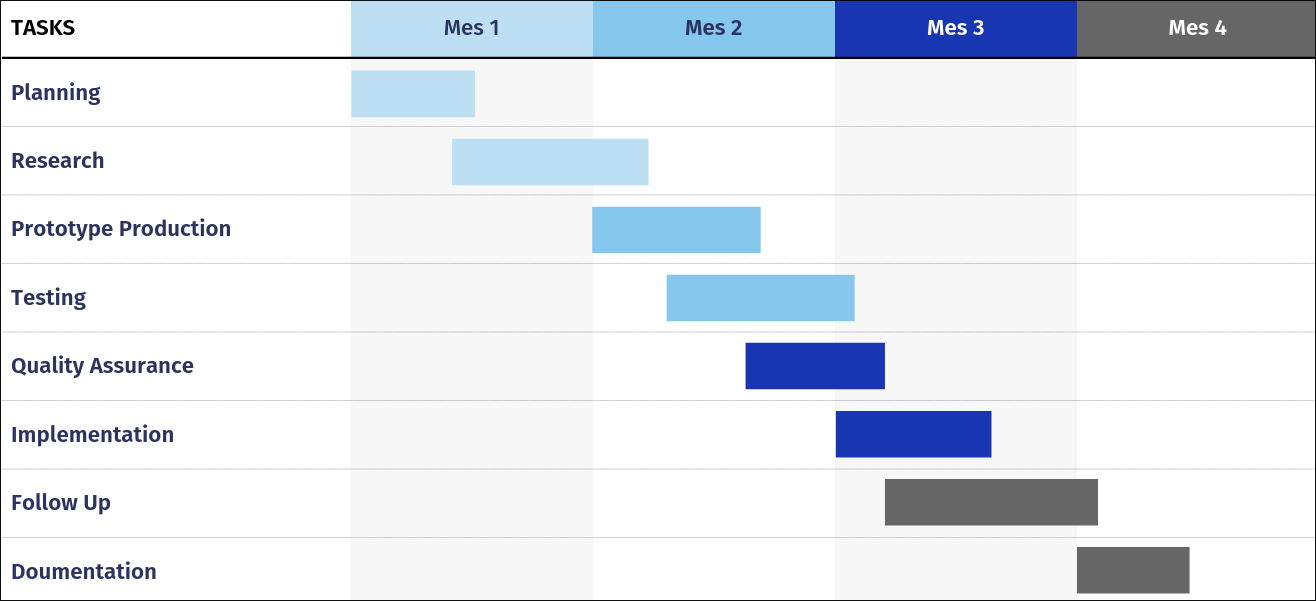
\includegraphics[width=\textwidth,keepaspectratio]{2025-04-18_16-03-51_screenshot.png}
    \caption{Diagrama de Gantt}
    \label{fig:enter-label}
\end{figure}



\subsection{Mecanismos de Monitoramento e Elaboração de Relatórios}
% descreve os relatórios de gerência que devem ser produzidos, quando e quais mecanismos de monitoramento são utilizados

\section{Projeto do Sistema}
% “Como fazer?” (arquitetura e modelos do sistema)

\newpage
\section{Protótipo de Interface}
% Projeto de tela e relatórios para ilustrar a solução

\newpage
\section{Conclusão}

\newpage
\renewcommand{\refname}{Bibliografia}
\begin{thebibliography}{09}
\bibitem{ibge-2022} INSTITUTO BRASILEIRO DE GEOGRAFIA E ESTATÍSTICA (IBGE). 
\textbf{Censo Demográfico 2022: São José do Rio Preto}. 
2022. 
Disponível em: \url{https://www.ibge.gov.br/cidades-e-estados/sp/sao-jose-do-rio-preto.html}. 
Acesso em: 20 abr. 2025.

\bibitem{} %{title} %author name here
\textbf{}. %text here

\bibitem{} %{title} %author name here
\textbf{}. %text here

\end{thebibliography}
\end{document}
